
\documentclass{article}
\usepackage{tikz}
\usepackage{float}
\usepackage{enumerate}
\usepackage{amsmath}
\usepackage{amsthm}
\usepackage{bm}
\usepackage{indentfirst}
\usepackage{siunitx}
\usepackage[utf8]{inputenc}
\usepackage{graphicx}
\graphicspath{ {Images/} }
\usepackage{float}
\usepackage{mhchem}
\usepackage{chemfig}
\allowdisplaybreaks

\title{6.041 Problem Set 6}
\author{Robert Durfee - R02}
\date{October 16, 2018}

\begin{document}

\maketitle

\section*{Problem 1}

\textit{Random variables $X$ and $Y$ have the joint PDF shown below:}

\begin{center}
    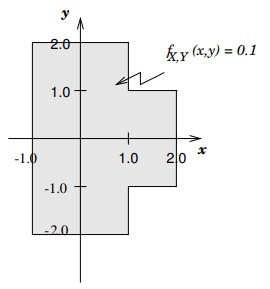
\includegraphics[scale=1]{Images/P1.PNG}
\end{center}

\subsection*{Part A}

\textit{Prepare neat, fully labeled sketches of $f_X(x)$, $f_Y(y)$,
$f_{Y|X}(y \mid x)$, and $f_{X|Y}(x \mid y)$.}

\bigbreak

The joint PDF described in the diagram is
$$ f_{X,Y}(x, y) = \begin{cases}
    0.1 & x \in [-1, 1]\, \mathrm{and}\, y \in [-2, 2] \\
    0.1 & x \in [1, 2]\, \mathrm{and}\, y \in [-1, 1] \\
    0 & \mathrm{otherwise}
\end{cases} $$

The marginal PDF for $X$ is
$$ f_X(x) = \begin{cases}
    0.4 & x \in [-1, 1] \\
    0.2 & x \in [1, 2] \\
    0 & \mathrm{otherwise}
\end{cases} $$

\begin{center}
    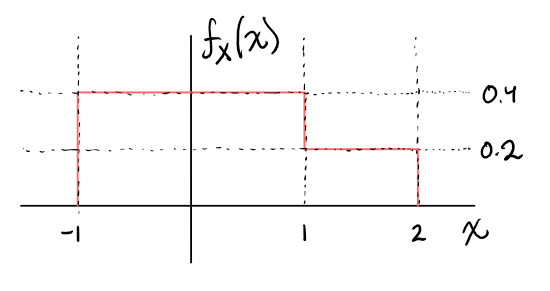
\includegraphics[scale=0.5]{Images/P1Ai.PNG}
\end{center}

The marginal PDF for $Y$ is
$$ f_Y(y) = \begin{cases}
    0.2 & y \in [-2, -1] \cup [1, 2] \\
    0.3 & y \in [-1, 1] \\
    0 & \mathrm{otherwise}
\end{cases} $$

\begin{center}
    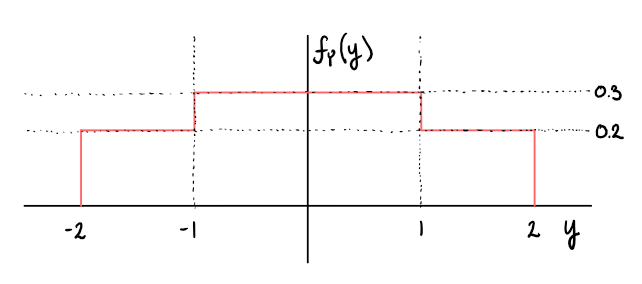
\includegraphics[scale=0.5]{Images/P1Aii.PNG}
\end{center}

The conditional PDF's for $X$ are
$$ f_{X|Y}(x \mid Y = y) = \begin{cases}
    1/3 & x \in [-1, 2] \\
    0 & \mathrm{otherwise}
\end{cases}\, \forall y \in [-1, 1]$$

\begin{center}
    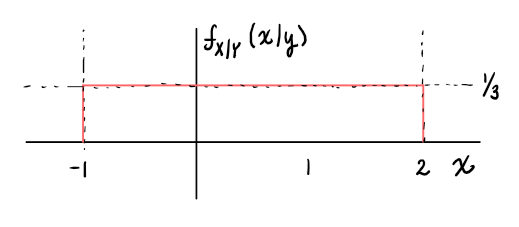
\includegraphics[scale=0.5]{Images/P1Aiii.PNG}
\end{center}

$$ f_{X|Y}(x \mid Y = y) = \begin{cases}
    1/2 & x \in [-1, 1] \\
    0 & \mathrm{otherwise}
\end{cases}\, \forall y \in [-2, -1] \cup [1, 2] $$

\begin{center}
    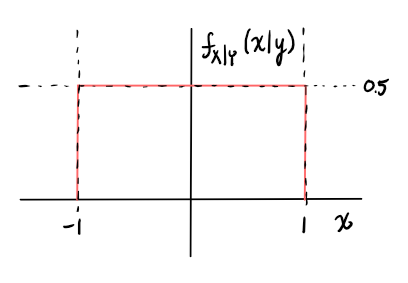
\includegraphics[scale=0.5]{Images/P1Aiv.PNG}
\end{center}

The conditional PDF's for $Y$ are
$$ f_{Y|X}(y \mid X = x) = \begin{cases}
    1/4 & y \in [-2, 2] \\
    0 & \mathrm{otherwise}
\end{cases}\, \forall x \in [-1, 1] $$

\begin{center}
    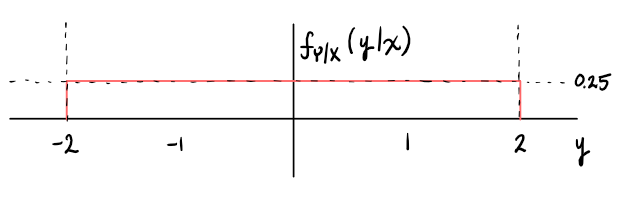
\includegraphics[scale=0.5]{Images/P1Av.PNG}
\end{center}

$$ f_{Y|X}(y \mid X = x) = \begin{cases}
    1/2 & y \in [-1, 1] \\
    0 & \mathrm{otherwise}
\end{cases}\, \forall x \in [1, 2] $$

\begin{center}
    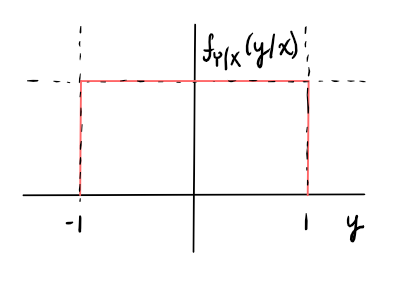
\includegraphics[scale=0.5]{Images/P1Avi.PNG}
\end{center}

\subsection*{Part B}

\textit{Are $X$ and $Y$ independent?}

\bigbreak

Let $y = 0.5$ and $x = 0.5$. Then the following are true
$$ f_{X,Y}(0.5, 0.5) = 0.1 $$
$$ f_X(0.5) = 0.4 $$
$$ f_Y(0.5) = 0.3 $$
The test for independence
$$ f_{X,Y}(x, y) = f_X(x) f_Y(y)\, \forall x, y $$
However,
$$ 0.1 \neq 0.4 \cdot 0.3 $$
Therefore, $X$ and $Y$ are not independent.

\subsection*{Part C}

\textit{Find $f_{X,Y|A}(x, y)$, where the event $A$ corresponds to points
$(x, y)$ within the unit circle centered at the origin.}

\bigbreak

The definition for the conditioning on an event
$$ f_{X,Y|\{X,Y \in A\}}(x, y) = \begin{cases}
    f_{X,Y}(x, y) / P(\{X, Y \in A\}) & x, y \in A \\
    0 & \mathrm{otherwise}
\end{cases} $$
The entire region of the unit circle overlaps with the joint PDF. Since the
joint PDF is uniformly distributed, so is the unit circle. Therefore, the
probability of event $A$ is the area of the unit circle times the value of
the joint PDF of $X$ and $Y$.
$$ P(\{X, Y \in A \}) = 0.1 \cdot \pi $$

Therefore, the conditional joint PDF is
$$ f_{X,Y|\{X,Y \in A\}}(x, y) = \begin{cases}
    1/\pi & x, y \in x^2 + y^2 \leq 1 \\
    0 & \mathrm{otherwise}
\end{cases} $$

\subsection*{Part D}

\textit{Find $E[X \mid Y = y]$ and $\mathrm{var}(X \mid Y = y)$.}

\bigbreak

From the definition of conditional expectation
$$ E[X \mid Y = y] = \int x f_{X|Y}(x \mid y) dx $$
Therefore, the conditional expectation of $X$ for $y \in [-1, 1]$ is
\begin{align*}
    E[X \mid Y = y] &= \int\limits_{-1}^2 \frac{x}{3} dx \\
    &= \left( \frac{x^2}{6} \right)_{-1}^2 \\
    &= \frac{2^2}{6} - \frac{(-1)^2}{6} \\
    &= \frac{1}{2}
\end{align*}
The conditional expectation of $X$ for $y \in [-2, -1] \cup [1, 2]$ is
\begin{align*}
    E[X \mid Y = y] &= \int\limits_{-1}^1 \frac{x}{2} dx \\
    &= \left( \frac{x^2}{4} \right)_{-1}^1 \\
    &= \frac{1^2}{2} - \frac{(-1)^2}{2} \\
    &= 0
\end{align*}
Therefore, the complete conditional expectation of $X$ is
$$ E[X \mid Y = y] = \begin{cases}
    1/2 & y \in [-1, 1] \\
    0 & y \in [-2, -1] \cup [1, 2]
\end{cases} $$

From the definition of variance
$$ \mathrm{var}(X \mid Y = y) = E[X^2 \mid Y = y] - E[X \mid Y = y]^2 $$
The second term can be determined directly from the expectation above
$$ E[X \mid Y = y]^2 = \begin{cases}
    1/4 & y \in [-1, 1] \\
    0 & y \in [-2, -1] \cup [1, 2]
\end{cases} $$
The first term can be calculated from the definition of expectation
$$ E[g(X) \mid Y = y] = \int g(x) f_{X|Y}(x \mid y) dx $$
Therefore, the conditional expectation of $X^2$ for $y \in [-1, 1]$ is
\begin{align*}
    E[X^2 \mid Y = y] &= \int\limits_{-1}^2 \frac{x^2}{3} dx \\
    &= \left( \frac{x^3}{9} \right)_{-1}^2 \\
    &= \frac{2^3}{9} - \frac{(-1)^3}{9} \\
    &= 1
\end{align*}
The conditional expectation of $X^2$ for $y \in [-2, -1] \cup [1, 2]$ is
\begin{align*}
    E[X^2 \mid Y = y] &= \int\limits_{-1}^1 \frac{x^2}{2} dx \\
    &= \left( \frac{x^3}{6} \right)_{-1}^1 \\
    &= \frac{1^3}{6} - \frac{(-1)^3}{6} \\
    &= \frac{1}{3}
\end{align*}
Therefore, the complete conditional expectation of $X^2$ is
$$ E[X^2 \mid Y = y] = \begin{cases}
    1 & y \in [-1, 1] \\
    1/3 & y \in [-2, -1] \cup [1, 2]
\end{cases} $$
Back to the definition of variance, the conditional variance is
$$ \mathrm{var}(X \mid Y = y) = \begin{cases}
    3/4 & y \in [-1, 1] \\
    1/3 & y \in [-2, -1] \cup [1, 2]
\end{cases} $$

\section*{Problem 2}

\textit{Consider the following problem and a purported solution. Either
declare the solution to be correct or explain the flaw.}

\bigbreak

\textit{\textbf{Question:} Let $X$ and $Y$ have the joint density}
$$ f_{X,Y}(x, y) = \begin{cases}
    1 & x \in [0, 1]\, \mathrm{and}\, y \in [x, x + 1] \\
    0 & \mathrm{otherwise}
\end{cases} $$
\textit{Find $f_X(x)$, $f_Y(y)$, and $f_{Y|X}(y \mid x)$. Are $X$ and $Y$
independent?}

\bigbreak

\textit{\textbf{Solution:}}
$$ f_X(x) = \int f_{X,Y}(x, y) dy = \int\limits_x^{x + 1} 1 \cdot dy = 1 $$
$$ f_Y(y) = \int f_{X,Y}(x, y) dx = \int\limits_0^1 1 \cdot dx = 1 $$
$$ f_{Y|X}(y \mid x) = \frac{f_{X,Y}(x, y)}{f_X(x)} = \frac{1}{1} = 1 $$
\textit{Since $f_{Y|X}(y \mid x)$ does not depend on $x$, we have that $X$
and $Y$ are independent. Alternatively, $X$ and $Y$ are independent because
$f_{X,Y}(x, y) = f_X(x) f_Y(y)$.}

\bigbreak

The provided solution is not correct. The error arises in the calculation of
the marginal PDF of $Y$. The correct marginal PDF of $Y$ is
$$ f_Y(y) = \begin{cases}
    \int\limits_0^y f_{X,Y}(x, y) dx & y \in [0, 1] \\
    \int\limits_{y - 1}^1 f_{X,Y}(x, y) dx & y \in [1, 2] \\
    0 & \mathrm{otherwise}
\end{cases} $$
Solving the first integral
\begin{align*}
    \int\limits_0^y 1 \cdot dx &= \left( x \right)_0^y \\
    &= y - 0 \\
    &= y
\end{align*}
Solvign the second integral
\begin{align*}
    \int\limits_{y - 1}^1 1 \cdot dx &= \left( x \right)_{y - 1}^1 \\
    &= 1 - (y - 1) \\
    &= 2 - y
\end{align*}
Therefore, the correct PDF for $Y$ is
$$ f_Y(y) = \begin{cases}
    y & y \in [0, 1] \\
    2 - y & y \in [1, 2] \\
    0 & \mathrm{otherwise}
\end{cases} $$

Now, checking the conditional for independence
$$ f_{X,Y}(x, y) = f_X(x) f_Y(y) $$
Let $x = 0.5$ and $y = 0.5$. Then the following is true
$$ f_{X,Y}(0.5, 0.5) = 1 $$
$$ f_X(0.5) = 1 $$
$$ f_Y(0.5) = 0.5 $$
However,
$$ 1 \neq 1 \cdot 0.5 $$ 
Therefore, $X$ and $Y$ are not independent.

\section*{Problem 3}

\textit{Random variables $X$ and $Y$ are independent and are described by the
probability density functions $f_X(x)$ and $f_Y(y)$:}
$$ f_X(x) = \begin{cases}
    1 & x \in (0, 1] \\
    0 & \mathrm{otherwise}
\end{cases} $$
$$ f_Y(y) = \begin{cases}
    1 & y \in (0, 1] \\
    0 & \mathrm{otherwise}
\end{cases} $$
\textit{Stations $A$ and $B$ are connected by two} parallel \textit{message
channels. One message from $A$ to $B$ is sent over each of the channels at
the same time. Random variables $X$ and $Y$ represent the message delays in
hours over parallel channels $1$ and $2$, respectively.}

\textit{A message is considered ``received'' as soon as it arrives on any one
channel and it is considered ``verified'' as soon as it has arrived over both
channels.}

\subsection*{Part A}

\textit{Determine the probability that a message is received within $15$
minutes after it is sent.}

\bigbreak

The desired probability is $P(\{X \leq 1/4\} \cup \{Y \leq 1/4\})$. Using the
inclusion-exclusion principle, the probability is the same as
$$ P(\{X \leq 1/4\}) + P(\{Y \leq 1/4\}) - P(\{X \leq 1/4\} \cap \{Y \leq
1/4\}) $$

The marginal CDFs of $X$ and $Y$ and joint CDF of $X$ and $Y$ are
$$ F_X(x) = x $$
$$ F_Y(y) = y $$
$$ F_{X,Y}(x, y) = xy $$

Using the CDFs,
\begin{align*}
    P(\{X \leq 1/4\} \cup \{Y \leq 1/4\}) &= F_X(1/4) + F_Y(1/4) - F_{X,Y}(1/4) \\
    &= \frac{1}{4} + \frac{1}{4} - \frac{1}{16} \\
    &= \frac{7}{16} 
\end{align*}

\subsection*{Part B}

\textit{Determine the probability that the message is received but not
verified within $15$ minutes after it is sent.}

\bigbreak

Let $A = \left(\{X \leq 1/4\} \cap \{Y \geq 1/4\}\right) \cup \left(\{Y \leq
1/4\} \cap \{X \geq 1/4\}\right)$. Thus, the probability desired is
$$ P(\{X \leq 1/4\}) + P(\{Y \leq 1/4\}) - 2 P(\{X \leq 1/4\} \cap \{Y \leq
1/4\}) $$

Using the CDFs,
\begin{align*}
    P(A) &= F_X(1/4) + F_Y(1/4) - 2 F_{X,Y}(1/4) \\
    &= \frac{1}{4} + \frac{1}{4} - \frac{2}{16} \\
    &= \frac{3}{8} 
\end{align*}

\subsection*{Part C}

\textit{Let $T$ represent the time in hours between transmission at $A$ and
verification at $B$. Determine the CDF $F_T(t)$, and then differentiate it to
obtain the PDF $f_T(t)$.}

\bigbreak

The random variable $T = |X - Y|$. From the joint PDF given, the probability
$P(|X - Y| > t)$ can be determined through the integral
\begin{align*}
    \int\limits_t^1\int\limits_0^{x - t} &f_{X,Y}(x, y) dy dx +
    \int\limits_0^{1 - t}\int\limits_{x + t}^1 f_{X,Y}(x, y) dy dx \\
    &= \int\limits_t^1\int\limits_0^{x - t} dy dx + \int\limits_0^{1 -
    t}\int\limits_{x + t}^1 dy dx \\
    &= \int\limits_t^1 \left(y\right)_0^{x - t} dx + \int\limits_0^{1 - t} \left(y\right)_{x + t}^1 dx \\
    &= \int\limits_t^1 (x - t) dx + \int\limits_0^{1 - t} (1 - x - t) dx \\
    &= \left(\frac{x^2}{2} - tx\right)_t^1 + \left(x - \frac{x^2}{2} - xt\right)_0^{1 - t} \\
    &= \left(\frac{1^2}{2} - t\right) - \left(\frac{x^2}{2} - t^2\right) + \left(\left(1 - t\right) - \frac{(1 - t)^2}{2} - \left(1 - t\right) \cdot t \right) \\
    &= \frac{1}{2} - t - \frac{t^2}{2} + t^2 + 1 - t - \frac{(1 - t)^2}{2} - t + t^2 \\
    &= -2t + t^2
\end{align*}
Flipping this,
$$ P(|X - Y| \leq t) = 1 - P(|X - Y| > t) $$
Therefore, the CDF for $T$ is given by
$$ F_T(t) = 2t - t^2 $$
Taking the derivative, the PDF for $T$ is given by
$$ f_T(t) = 2 - 2t $$

\subsection*{Part D}

\textit{If the attendant at $B$ leaves for a $15$-minute coffee break right
after the message is received, what is the probability that he is present at
the proper time for verification?}

\bigbreak

The probability of receiving the message $15$ minutes after the receipt of
the message is the same as the probability that the time $T$ between receipt
and verification is greater than $15$ minutes.
$$ P(T \geq 1/4) = 1 - P(T \leq 1/4) $$
Using the CDF calculated above,
\begin{align*}
    P(T \geq 1/4) &= 1 - F_T(1/4) \\
    &= 1 - \left(\frac{2}{4} - \left(\frac{1}{4}\right)^2\right) \\
    &= 1 - \frac{8}{16} + \frac{1}{16} \\
    &= \frac{8}{16} - \frac{1}{16} \\
    &= \frac{9}{16}
\end{align*}
Therefore, the probability that the attendant receives the message is $ 9/16 $.

\subsection*{Part E}

\textit{The management wishes to have the maximum probability of having the
attendant present for} both \textit{reception and verification. Would they do
better to let him take his coffee break as described above or simply allow
him to go home $45$ minutes after transmission?}

\bigbreak

The probability of receiving and verifying the message $45$ minutes after
transmission is given by $P(\{X \leq 3/4\} \cap \{Y \leq 3/4\})$. Using the
joint CDF,
$$ F_{X,Y}(3/4, 3/4) = \frac{3}{4} \cdot \frac{3}{4} = \frac{9}{16} $$
Therefore, this is the same as the probability of verifying $15$ minutes
after receiving the message. The management can choose between either method.

\section*{Problem 4}

\textit{A defective coin minting machine produces coins whose probability of
heads is a random variable $P$ with PDF}
$$ f_P(p) = \begin{cases}
    2(1 - p) & p \in [0, 1] \\
    0 & \mathrm{otherwise}
\end{cases} $$
\textit{In essence, a specific coin produced by this machine will have a
fixed probability $P = p$ of giving heads, but you do not know initially what
that probability is. A coint produced by this machine is selected and tossed
repeatedly, with successive tosses assumed independent.}

\subsection*{Part A}

\textit{Find the probability that the first coin toss results in heads.}

\bigbreak

Using the definition of total probability,
$$ P(H_1) = \int f_P(p) P(H_1 \mid \{P = p\}) $$
The conditional probability for $H_1$ is simply $p$, therefore
\begin{align*}
    P(H_1) &= \int\limits_0^1 2 p (1 - p) dp \\
    &= \int\limits_0^1 (2 p - 2 p ^2) dp \\
    &= \left( p^2 - \frac{2p^3}{3} \right)_0^1 \\
    &= 1 - \frac{2(1)^3}{3} \\
    &= 1 - \frac{2}{3} \\
    &= \frac{1}{3}
\end{align*}

\subsection*{Part B}

\textit{Given that the first coin toss resulted in heads, find the
conditional PDF of $P$.}

\bigbreak

Using Bayes' theorem
$$ P(\{P = p\} \mid H_1) = \frac{P(H_1 \mid \{P = p\}) P(\{P = p\})}{P(H_1)} $$
This is the same as
$$ f_{P|H_1}(p) = \frac{P(H_1 \mid \{P = p\}) f_P(p)}{P(H_1)} $$
Using the information determined in Part A,
\begin{align*}
    f_{P|H_1}(p) &= \frac{2p(1 - p)}{1/3} \\
    &= 6p(1 - p)
\end{align*}
Therefore, the complete conditional PDF for $p$ is
$$ f_{P|H_1}(p) = \begin{cases}
    6p(1 - p) & p \in [0, 1] \\
    0 & \mathrm{otherwise}
\end{cases} $$

\subsection*{Part C}

\textit{Given that the first coin toss resulted in heads, find the
conditional probability of heads on the second toss.}

\bigbreak

Given that these two events are dependent through $p$,
$$ P(H_2 \mid H_1) = \int P(H_2 \mid H_1 \cap \{P = p\}) f_{P|H_1}(p) dp $$
Given that $P$ is already conditioned on $H_1$, this can be simplified
$$ P(H_2 \mid H_1) = \int P(H_2 \mid \{P = p\}) f_{P|H_1}(p) dp $$
Using the information determined in Parts A and B,
\begin{align*}
    P(H_2 \mid H_1) &= \int\limits_0^1 6 p^2 (1 - p) dp \\
    &= \int\limits_0^1 \left(6 p^2 - 6p^3\right) dp \\
    &= \left(\frac{6 p^3}{3} - \frac{6 p^4}{4} \right)_0^1 \\
    &= 2 - \frac{3}{2} \\
    &= \frac{1}{2}
\end{align*}

\section*{Problem 5}

\textit{Let $K$ be a discrete random variable with PMF}
$$ p_K(k) = \begin{cases}
    1/3 & k = 1 \\
    2/3 & k = 2 \\
    0 & \mathrm{otherwise}
\end{cases} $$
\textit{Conditional on $K = 1$ or $2$, random variable $Y$ is exponentially
distributed with parameter $1$ or $1/2$, respectively. Using Bayes' rule,
find the conditional PMF $p_{K|Y}(k \mid y)$.}

\bigbreak

Using Bayes' theorem for discrete and continuous random variables,
$$ p_{K|Y}(k \mid Y = y) = \frac{p_K(k) f_{Y|K}(y \mid K = k)}{\sum_k p_K(k)
f_{Y|K}(y \mid K = k)} $$
Substituting the definitions given for $K = 1$:
$$ p_{K|Y}(k \mid Y = y) = \frac{e^{-y}}{e^{-y} + e^{-y / 2}} $$
And for $K = 2$:
$$ p_{K|Y}(k \mid Y = y) = \frac{e^{-y / 2}}{e^{-y} + e^{-y / 2}} $$
Therefore, the complete conditional PMF for $K$ is:
$$ p_{K|Y}(k \mid Y = y) = \begin{cases}
    1 / (e^{y / 2} + 1) & k = 1 \\
    1 - 1 / (e^{y / 2} + 1) & k = 2 \\
    0 & \mathrm{otherwise}
\end{cases} $$

\end{document}